\documentclass{beamer} %[12pt]
\usepackage{xcolor}
%\usetheme{boadilla}
%\usetheme{malmoe}
%\usetheme{copenhagen}
%\usecolortheme{rose}
\usecolortheme{beaver}
\usepackage{pgf, graphics}
\usepackage{graphicx}
%\usepackage[left=3cm,top=3cm,right=3cm,nohead,nofoot]{geometry}
\usepackage{hyperref}
\usepackage{setspace}
\usepackage[square]{natbib}
\usepackage{amsmath}
\usepackage{amssymb}
\usepackage{verbatim}
\usepackage{color}
\usepackage{fancyvrb}
\usepackage{bbm}

\begin{filecontents}{ref.bib}
\end{filecontents}

%\usetheme{EastLansing}
%\usepackage{natbib}
\bibliographystyle{apalike}
% make bibliography entries smaller
%\renewcommand\bibfont{\scriptsize}
% If you have more than one page of references, you want to tell beamer
% to put the continuation section label from the second slide onwards
\setbeamertemplate{frametitle continuation}[from second]
% Now get rid of all the colours
\setbeamercolor*{bibliography entry title}{fg=black}
\setbeamercolor*{bibliography entry author}{fg=black}
\setbeamercolor*{bibliography entry location}{fg=black}
\setbeamercolor*{bibliography entry note}{fg=black}
% and kill the abominable icon
\setbeamertemplate{bibliography item}{}


\newcommand{\hl}[1]{\colorbox{yellow}{#1}}
\newcommand{\hlblue}[1]{\colorbox{green}{#1}}
\newcommand{\hlblu}[1]{\colorbox{cyan}{#1}}
\newcommand{\hlred}[1]{\colorbox{cyan}{#1}}
\newcommand{\hlre}[1]{\colorbox{pink}{#1}}
\newcommand{\hlgreen}[1]{\colorbox{pink}{#1}}
\newcommand{\hlgree}[1]{\colorbox{green}{#1}}



\DeclareMathOperator*{\argmax}{\arg\!\max}

\DeclareMathOperator*{\argmin}{\arg\!\min}


\newcommand{\specialcell}[2][c]{%
  \begin{tabular}[#1]{@{}c@{}}#2\end{tabular}}



%\setbeamersize{text margin left=.5cm,text margin right=.5cm}
\newenvironment{changemargin}[2]{%
  \begin{list}{}{%
    \setlength{\topsep}{0pt}%
    \setlength{\leftmargin}{#1}%
    \setlength{\rightmargin}{#2}%
    \setlength{\listparindent}{\parindent}%
    \setlength{\itemindent}{\parindent}%
    \setlength{\parsep}{\parskip}%
  }%
  \item[]}{\end{list}}
\setbeamertemplate{navigation symbols}{}%remove navigation symbols
\usepackage{color}
\newcommand{\hilight}[1]{\colorbox{yellow}{#1}}
\setbeamertemplate{footline}[page number]

\begin{document}


\title[dedup]{Interactive Graphics}


\author[Samuel L. Ventura]{\\
  \large{Sam Ventura\\Interactive Graphics}}
\institute[CMU Statistics]{Department of Statistics\\Carnegie Mellon University}
\date{\today}


\begin{frame}
	\maketitle

	
\end{frame}




\begin{frame}\frametitle{Introduction to Interactive Graphics}
	\small
	
	\textbf{Interactive Graphics:}
	\begin{itemize}
		\item Graphic that displays additional dimensions to the base visualization via some feature with which the user/viewer can control
		\item ``Dimension'' = variables/attributes, model changes, subsetting
	\end{itemize}
	
	
	\vskip 15 cm
	
\end{frame}



\begin{frame}\frametitle{Introduction to Interactive Graphics}
	\small
	
	\textbf{Interactive Graphics:}
	\begin{itemize}
		\item Graphic that displays additional dimensions to the base visualization via some feature with which the user/viewer can control
		\item ``Dimension'' = variables/attributes, model changes, subsetting
	\end{itemize}
	
	\vskip 1 cm
	
	\textbf{Types of Interactive Graphics:}
	\begin{itemize}
		\item Alt-text / ``hovering'':  Display additional features or information about an observation/group/category/etc via user's cursor control (mouse, tapping, etc)
		\item Filtering / subsetting (the data):  Updates graphic to show only \\a \emph{conditional} subset of the data
		\item Dynamic graphics / animation:  Not really ``interactive'', but add \\an extra dimension to the visualization (usually changes over time)
	\end{itemize}
	
	\vskip 10 cm
	
\end{frame}



\begin{frame}\frametitle{Dynamic $\neq$ Informative}
	\small
	\centering
	
	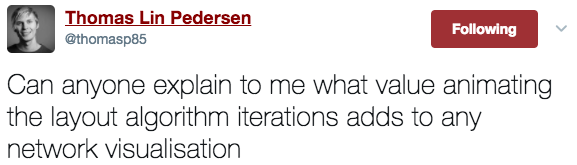
\includegraphics[width = 0.8\linewidth]{thomasp85-1.png}\\
	
	\vskip 1 cm
	
	
\includegraphics[width = 0.8\linewidth]{thomasp85-2.png}\\
	
	
\end{frame}




\begin{frame}\frametitle{Writing and Speaking About Interactive Graphics}
	\small
	
	Actions you should take when writing about / speaking about / presenting / demonstrating interactive graphics:
	
	\vskip 15 cm
	
\end{frame}



\begin{frame}\frametitle{Writing and Speaking About Interactive Graphics}
	\small
	
	Actions you should take when writing about / speaking about / presenting / demonstrating interactive graphics:
	
	\vskip 0.5 cm
	
	\begin{enumerate}
		\item Describe the base/initialized graphic
	\end{enumerate}
	
	
	\vskip 15 cm
	
\end{frame}



\begin{frame}\frametitle{Writing and Speaking About Interactive Graphics}
	\small
	
	Actions you should take when writing about / speaking about / presenting / demonstrating interactive graphics:
	
	\vskip 0.5 cm
	
	\begin{enumerate}
		\item Describe the base/initialized graphic

	\vskip 0.5 cm
	
		\item Use interactive features to demonstrate some interesting feature of the data!  (Something that you wouldn't otherwise see without the interactive features.)
	\end{enumerate}
	
	
	\vskip 15 cm
	
\end{frame}



\begin{frame}\frametitle{Writing and Speaking About Interactive Graphics}
	\small
	
	Actions you should take when writing about / speaking about / presenting / demonstrating interactive graphics:
	
	\vskip 0.5 cm
	
	\begin{enumerate}
		\item Describe the base/initialized graphic

	\vskip 0.5 cm
	
		\item Use interactive features to demonstrate some interesting feature of the data!  (Something that you wouldn't otherwise see without the interactive features.)
		
	\vskip 0.5 cm
	
		\item Demonstrate how to use the interactive features in doing so
	\end{enumerate}
	
	
	\vskip 15 cm
	
\end{frame}



\begin{frame}\frametitle{Writing and Speaking About Interactive Graphics}
	\small
	
	Actions you should take when writing about / speaking about / presenting / demonstrating interactive graphics:
	
	\vskip 0.5 cm
	
	\begin{enumerate}
		\item Describe the base/initialized graphic
		
		\vskip 0.5 cm
		
		\item Use interactive features to demonstrate some interesting feature of the data!  (Something that you wouldn't otherwise see without the interactive features.)
		
		\vskip 0.5 cm
		
		\item Demonstrate how to use the interactive features in doing so
		
		\vskip 0.5 cm
		
		\item Do NOT just demo interactive features because they're cool -- that's not enough! 
	\end{enumerate}
	
	
	\vskip 15 cm
	
\end{frame}




\begin{frame}\frametitle{Interactive Graphics in R}
	\small
	
	There are three ways to do interactive graphics in \texttt{R}
	
	\vskip 0.5 cm
	
	\begin{enumerate}
		\item \textbf{Plotly:}  \texttt{cpsievert.github.io/plotly\_book/} \\
		(Interface to JavaScript graphing library plotly.js)
		
		\vskip 0.5 cm
		
		\item \textbf{Shiny:}  \texttt{shiny.rstudio.com} \\
		(web application framework for \texttt{R})
		
		\vskip 0.5 cm
		
		\item \textbf{HTML Widgets:}  \texttt{www.htmlwidgets.org} \\
		(R interface to other JavaScript graphing tools)
		
	\end{enumerate}
	
	
	\vskip 15 cm
	
\end{frame}



\end{document}
